% !TEX encoding = UTF-8 Unicode
%%%%%%%%%%%%%%%%%%%%%%%%%%%%%%%%%%%%%%%%%%%%%%%%%%%%%%%%%%%%%%%%%%%%%%%%%%%%%%%%%%%%%%%%%%%%%%%%%%%%%%% 
%%
%%  This file is asmeconf-template.tex, a LaTeX template to format ASME Conference papers according to
%%  the requirements on ASME's conference web pages, and including hypertext support for the pdf.
%%
%%  This file is version 1.30 dated 2022/03/14
%%  
%%  As of version 1.11, this template defaults to ASME's newer conference guidelines first posted July 2019.
%% 			Those guidelines changed the requested author block formatting to be inline. 
%%			This LaTeX template continues to support the traditional grid format as a package option, [grid].
%%			Nomenclature now follows the abstract. Abstract text is set in italics.
%%
%%  Author: John H. Lienhard V
%%          Department of Mechanical Engineering
%%          Massachusetts Institute of Technology
%%          Cambridge, MA 02139-4307 USA
%%
%%  Class options include:
%%
%%          * Math options from M. Sharpe's newtxmath package: upright integrals [upint]; 
%%          *    [varvw] for a v and w that are better distinguished from Greek nu; and also 
%%          *    [subscriptcorrection, smallerops, varg, frenchmath, varbb, cmbraces, slantedGreek,...] 
%%			* 	 See newtx documentation for descriptions (at CTAN: http://ctan.org, v1.6 or higher is best).
%%
%%          * Options to: 	omit the ASME copyright footer [nofoot]; 
%%			*				use government employee copyright notice [govt];
%%			*				use government contractor copyright notice [contractor]
%%
%%          * An option to use the traditional grid arrangement of author names [grid].  
%%			*	 With this option, line breaks (\\) may be inserted into the address as needed. 
%%			*	 Author names that include commas should be enclosed in braces, e.g., {Joseph L. Smith, Jr.}.  
%%			*	 Authors may be grouped above a single affiliation using braces, e.g., {Henry Tudor, Catherine Parr}.
%%
%%          * An option to balance the heights of columns on the last page [balance]. 
%%          *    This option is NOT compatible with the [lineno] option.
%%
%%          * An option to include line numbers [lineno]. You must *run twice* for proper placement of the line numbers. 
%%			*	 The lineno package does not number titles, footnotes, captions, or tables.
%%          *    This option will disable balancing column height on final page if that option has been invoked.
%%          *    The lineno package won't always number the lines preceding displayed math in a paragraph because
%%          *    paragraph has not ended.  See that package's documentation for macros to address this problem, or
%%          *    just leave a blank line above the displayed equation while you are editing and then remove the 
%%          *    blank line and [lineno] option when you move to your final version.
%%
%%			* Options for PDF/A compliance. [pdf-a] will produce PDF/A-3u compliance with sRGB OutputIntent.
%%			*	 [pdfapart= 1 or 2 or 3] and [pdfaconformance= b or u] can enable levels 1b, 2b, 2u, and 3b.
%%			*    The most recent versions of LaTeX (2021 and later) are moving toward integrated support for pdf-a, 
%%			*    through \DeclareDocumentMetadata{..}. The asmeconf class supports these new features, which can 
%%			*	 replace the aforementioned class options. (An up-to-date LaTeX installation is required to use this.)
%%
%%          * Many options for calligraphic, script, and fraktur fonts from the mathalfa package; the
%%          *    example shown here is: [mathalfa=cal=boondoxo] to use a Boondox font for \mathcal.
%%          *    Some other options for cal are: dutchcal, zapfc, cm (default), euler,...
%%          *    frak (fraktur), bb (blackboard bold), scr (script) may also be chosen this way.
%%			*	 For details, refer to mathalfa documentation (at CTAN: http://ctan.org).
%%
%%          * Option to use superiors font from newtxtext for footnotes [nodefaultsups] and
%%          *    for slightly larger small capitals, [largesc], also from newtxtext.
%%
%%          * An option to allow hyphenation of the typewriter font [hyphenate], from inconsolata package.
%%          *    Hyphenation is normally suppressed for typewriter mode because it is often used for code.
%%			*	 To replace the default variable word spacing by monospacing, use the option [mono].
%%			*	 To get a zero without a slash, use [var0]
%%
%%          * Options (used by the babel package) to include passages in languages other than English (e.g., a translation 
%%			*    of the abstract). Languages are called as options, e.g. [french], [spanish], [greek], [russian], etc. 
%%			*    Language support is greatest when running LuaLaTeX with the [fontspec] option.
%%			*    See Appendix B for details.
%%
%%  The use of commands defined or modified by the asmeconf class is illustrated throughout this file. In particular, 
%%  ASME requires capitalized, sans-serif section headings, and as a result some care is needed when using macros 
%%  in section headings, as also illustrated below.
%%
%%  Use an up-to-date and complete installation of LaTeX, such as TeX Live 2020 or later. Errors may occur with old set-ups.
%%
 %=========================================================
%% 
%% LICENSE: 
%%
%% Copyright (c) 2022 John H. Lienhard
%%
%% Offered under the MIT license: https://ctan.org/license/mit 
%%
%%%%%%%%%%%%%%%%%%%%%%%%%%%%%%%%%%%%%%%%%%%%%%%%%%%%%%%%%%%%%%%%%%%%%%%%%%%%%%%%%%%%%%%%%%%%%%%%%%%%%%% 

%% New pdf management code (June 2021); with this, the class option [pdf-a] can be omitted.
%% This change to the LaTeX kernel is being phased-in by the LaTeX3 team. Can delete if it gives you trouble.
%% Under LuaLaTeX, choose pdfstandard=A-3b (and be cautious when loading extra fonts)

%\RequirePackage{pdfmanagement-testphase}%
%   \DocumentMetadata{%
%		pdfstandard=A-3b,% A-2b, A-2u, A-3b, or A-3u
%		pdfversion=1.7,
%		lang=en-US,
%	}%

%%%%%%%%%%%%%%%%%%%%%%%%%%%%%%%%%%%%%%%%%%%%%%%%%%%%%%%%%%%%%%%%%%%%%%%%%%%%%%%%%%%%%%%%%%%%%%%%%%%%%%%

%% Class options are described above. Change these options as desired. 
%%		If you are not using the language options, remove them (together with Appendices B and C)
%%	 	Remove the [colorlinks] option before *final* submission to ASME, to get black text for printing,
%%		but keep that option for other uses.
 
\documentclass[balance,upint,subscriptcorrection,varvw,nofoot, mathalfa=cal=boondoxo,spanish,french,vietnamese,russian,greek,pdf-a,fontspec,colorlinks]{asmeconf}
%%%%%  pdf metadata  %%%%%%%%%%%%%%%%%%%%%%%%%%%%%%%%%%%%%%%%%%%%%%%%%%%%%%%%%%%%%%%%%%%%%%%%%%%%%%%%%%
\hypersetup{%
	pdfauthor={John H. Lienhard},                       		      % <=== change to YOUR name[s]!
	pdftitle={ASME Conference Paper LaTeX Template},                  % <=== change to YOUR pdf file title
	pdfkeywords={ASME conference paper, LaTeX template, BibTeX style},% <=== change to YOUR pdf keywords
	pdfsubject = {Describes the asmeconf LaTeX template},			  % <=== change to YOUR subject
%	pdfurl={https://ctan.org/pkg/asmeconf},% may delete
	pdflicenseurl={https://ctan.org/pkg/asmeconf},% may delete
}

%%%%%%%%%%%%%%%%%%%%%%%%%%%%%%%%%%%%%%%%%%%%%%%%%%%%%%%%%%%%%%%%%%%%%%%%%%%%%%%%%%%%%%%%%%%%%%%%%%%%%%%
\usepackage{minted}
\makeatletter
\@namedef{T1/zi4/m/it}{<->ssub*zi4/m/n}
\begin{document}

% Change these fields to the right content for your conference.
% You can comment these out if for some reason you don't want a header.
% Use title case (first letters capitalized), not all capitals

% \ConfName{Proceedings of the ASME 2022\linebreak International Mechanical Engineering Congress and Exposition}
% \ConfAcronym{IMECE2022}
% \ConfDate{October 30--November 3, 2022} % update 
% \ConfCity{Columbus, OH} % update 
% \PaperNo{IMECE2022-XXXX}

% Units of measure (e.g., cm) and other specialty lowercase terms in the title should be 
%   enclosed in \NoCaseChange{...} to maintain lower case type
%   LaTeX will automatically set the rest of the title in all capital letters.

\title{Stereo Camera and Solid State Lidar Object Detection on Small Delivery Robot} % <=== replace with YOUR title
%\title{Place Title Here: Place Subtitle After Colon} 
 
%   Put author names into the order you want. Use the same order for affiliations.
%   \affil{#} tags the author's affiliation to the address in \SetAffiliation{#}.
%   No space between last name and \affil{#}, separate names with commas.
%
%	For a sole author or a single affiliation for all authors, {#} may be left empty, as \affil{} and \SetAffiliation{} (but not with [grid] option!)
%
%   \CorrespondingAuthor{email} follows that author's affiliation, no spaces.  
%   If multiple corresponding authors, put both email addresses in the same command and place after both authors.
%
%   \JointFirstAuthor, if applicable, follows the affiliation of the relevant authors, no spaces.

\SetAuthors{%
	Jiarun Wei\affil{1}\JointFirstAuthor, 
	Ding Zhao\affil{2}\JointFirstAuthor
	}

\SetAffiliation{1}{Carnegie Mellon University, Pittsburgh, PA}
\SetAffiliation{2}{Carnegie Mellon University, Pittsburgh, PA}

%	Note: Luis and Maria are not real people.  Henry and Catherine have been dead for >450 years.

%	To switch from inline author names to gridded names, use the [grid] option.

\maketitle

%%% Use this footnote for tracking various versions of your draft. Change text to suit your own needs. 
%%% \date{..} calls the same command. 
% \versionfootnote{Documentation for \texttt{asmeconf.cls}: Version~\versionno, \today.}% <=== Delete before final submission.


%%% Change these to your keywords.  Keywords are automatically printed at the end of the abstract.
%%% This command MUST COME BEFORE the end of the abstract.
%%% If you don't want keywords, leave the argument of \keywords{} empty (or use the abstract* environment)

\keywords{Object detection, Computer Vision, Solid-state Lidar, Autonomous Delivery}

%%%%%  End of fields to be completed. Now write your paper. %%%%%%%%%%%%%%%%%%%%%%%%%%%%%%%%%%%%%%%%%%%


%%%%%  ABSTRACT  %%%%%%%%%%%%%%%%%%%%%%%%%%%%%%%%%%%%%%%%%%%%%%%%%%%
%%
%% Abstract should be 200 words or less
\begin{abstract}

Stereo camera is popular in object detection due to its dense data. It works by matching
the key points of the left and right images, using the geometric constraints to calculate
the depth map, and then feed these into a neural network. Due to the geometric
constraints, it only works for a certain range of objects and is unstable for some objects.
Here we present a demo to stabilize the detection using solid state lidars, which is a very
cost efficient solution especially for small and slow robots.
\end{abstract}

%%%%%%%%%  NOMENCLATURE (OPTIONAL) %%%%%%%%%%%%%%%%%%%%%%%%%%%%%%%%%
%%
%% To change space between the symbols and  definitions, use \begin{nomenclature}[Xcm] where X is a number 
%% The unit cm can be replaced by any LaTeX unit of dimension: pt, in, ex, em, pc, etc.
%% Default is 2em.
%% \EntryHeading{..} produces an italicized subheading in the nomenclature list, e.g., \EntryHeading{Greek letters}




%%%%%%%%%  BODY OF PAPER %%%%%%%%%%%%%%%%%%%%%%%%%%%%%%%%%

\section{Introduction}
In the industry of autonomous delivery, it is widely proved that the perception part of the autonomous system is the bottle neck. Due to the complicated environment of the real world, it is hard for the vehicle to navigate around. The vehicle it self must get a very detailed and precise information of what the surrounding is like.

In order to achieve that, 2 types of sensors are invented, the cameras and the lidars, both of which uses the lights to percept the surrounding. However, both camera and lidars have pros and cons are always used together to get rid of the disadvantages of each other. The camera is similar to human's eyes. It captures the lights reflected from the surrounding objects projected on a 2D plane. However the reflectional lights can be confusing because the image captured by the camera and the real environment is not necessary  one-to-one mapping. On contrary, the lidars launch lights it self and calculates the distance according to the time interval between the launch time and the receiving time. This is very precise in terms of the depth measurement, however lacks of semantics information due to the absence of colors. 

Great efforts of the developmet of the lidars has been made to achieve a higher perception accuracy. For example, the velodyne lidar is the most important sensor. It is used to detect objects in the environment with multiple threads. However, due to the demand of high speed of real vehicles, the density of its threads are required to be very high. For small delivery robots, many researchers directly deploys the velodyne lidar, which might not be necessary given the speed and height of those small vehicles. 

In this paper, a novel method to utilize a very cost efficient solid state lidar combined with stereo camera to stabilize the detection of objects on small delivery robots is proposed. We also established a prototype of the small autonomous delivery robot system and demonstrate the system's performance. This robot can navigate across within certain area within CMU campus given arbitrary initial position and target position. It is about half a person tall with omnidirectional wheels that can carry a small parcel.  

\section{System Design}
As is shown in figure \ref{sys}, the delivery robot can be divided into 6 parts: stereo camera, router, battery, solid-state lidar and the processor. The part list is shown in table \ref{parts}.
\begin{table}[!ht]
    \centering
    \begin{tabular}{p{0.2\linewidth} p{0.2\linewidth} p{0.2\linewidth} p{0.2\linewidth}}
    \hline
        ID & Category & Part & Qty \\ \hline
        SAFEAI001 & Joystick Controllers & Mecanum Wheel Controller & 1 \\ 
        SAFEAI002 & Joystick Controllers & Regular Wheel Controller & 1 \\ 
        SAFEAI003 & LiDARs & Solid-state Livox Mid-70 Lidars & 3 \\ 
        SAFEAI004 & LiDARs & SLAMTec Lidars & 2 \\ 
        SAFEAI005 & Cameras & ZED Camera & 2 \\ 
        SAFEAI006 & Power Supplies & Krisdonia Power Bank & 1 \\ 
        SAFEAI007 & Power Supplies & MAXOAK Power Bank & 2 \\ 
        SAFEAI008 & Computers & AGX Jetson & 2 \\ 
        SAFEAI009 & Internet communications & Router & 2 \\ \hline
    \end{tabular}
	\caption{Part list}\label{parts}
\end{table}


\paragraph{Stereo camera} The stereo camera is used for the detection of dynamic obstacles such as human and vehicles. Though the depth obtained by the stereo camera is not as accurate as the lidar, its object detection ability is a lot more better due to the RGB triple input channels.
\paragraph{Solid-state lidar} The lidar is used in multiple tasks: mapping, localization and object detection. During the mapping task, the lidar scans around a certain area and reconstructs a 3D point cloud map of the surroundings. In the localization task, the lidar scans forward and locate the robot using a Normal Distribution Transform matching method, which matches the distribution of point cloud of previous map and the current scanning. In the object detection task, the lidar gets the semantics of the current scanning.
\paragraph{Processor} The processor is used to process the data obtained by the lidar and the stereo camera. The processor uses a neural network that can process the data and generate the semantics of the current scanning.
\paragraph{Battery} There are 2 types of batteries, one is the chassis battery which is used to power the chassis and move the whole vehicle. Another is the power banks which are used to power the processor, lidars, and the router. The rated power of the chassis and the power banks are different so they have to be separated.
\paragraph{Router} The router is used to connect the lidar and the processor. It plays an important role in the synchronization process between the lidar and the processor.


\section{Methods}

Stereo R-CNN based 3D Object Detection \cite{DBLP:journals/corr/abs-1902-09738} is deployed in the system. It can be decomposed into several parts: feature extraction, reigion proposal, reigion of intersection alignment, keypoint prediction and 3D bounding box estimation, which involves deep neural networks such as ResNet and binocular geometric constraints. In the following experiment, the lidar point clouds are used to verify the detection.
\paragraph{Feature extraction} The ResNet \cite{7780459} is one of the most commonly used feature extraction methods. Its architecture is shown in figure \ref{res}. Unlike the regular sequential CNNs, the ResNet adds the forward propagation from the input of each blocks directly to their output. 
\paragraph{Reigion proposal} The Faster R-CNN network\cite{DBLP:journals/corr/RenHG015} is used to propose the regions of interest. It can be divided into 3 steps: anchor generation, foreground-background classification and bounding box regression. The anchors are generated in the feature space of the output of the feature extraction backbone. They are mapped back to the image regions according to the aspect ratios and scales, which are all trainable parameters. 
\paragraph{Region of intersection alignment} Given the ground truth bounding boxes, the candidate boxes are further classified into foreground or background using the overlapping ratio with the ground truth as criterion. The ground truth is a heavy work which requirs a lot of human resources.
\paragraph{Keypoint prediction and 3D bounding box estimation} After the region of intersection is calculated, the network can do a regression to estimate the position and size of the bounding boxes using backpropagation.


\begin{figure}
\centering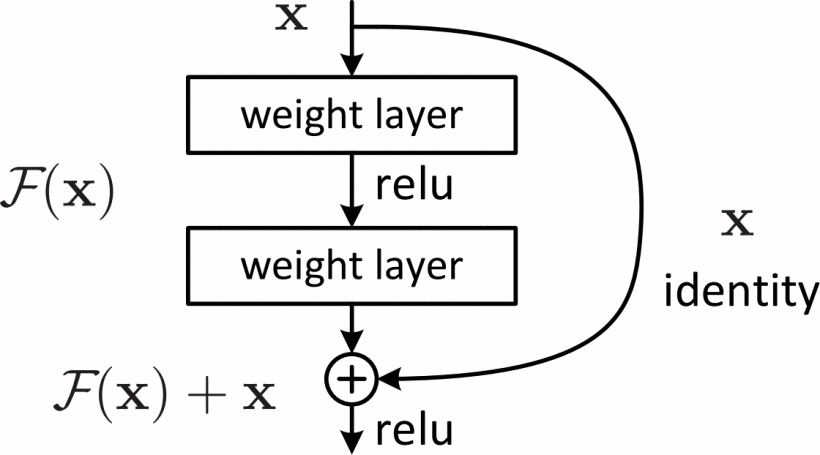
\includegraphics[width=0.7\linewidth]{resnet.png}
\caption{ResNet block}\label{res}
\end{figure}

%%%%%%%%%%%%%%%%%%%%%%%%%%%%%%%%%%%%%%%%%%%%%%%%%%%%%%%%%%%

\section{Experiment}
\begin{figure*}
	\center
	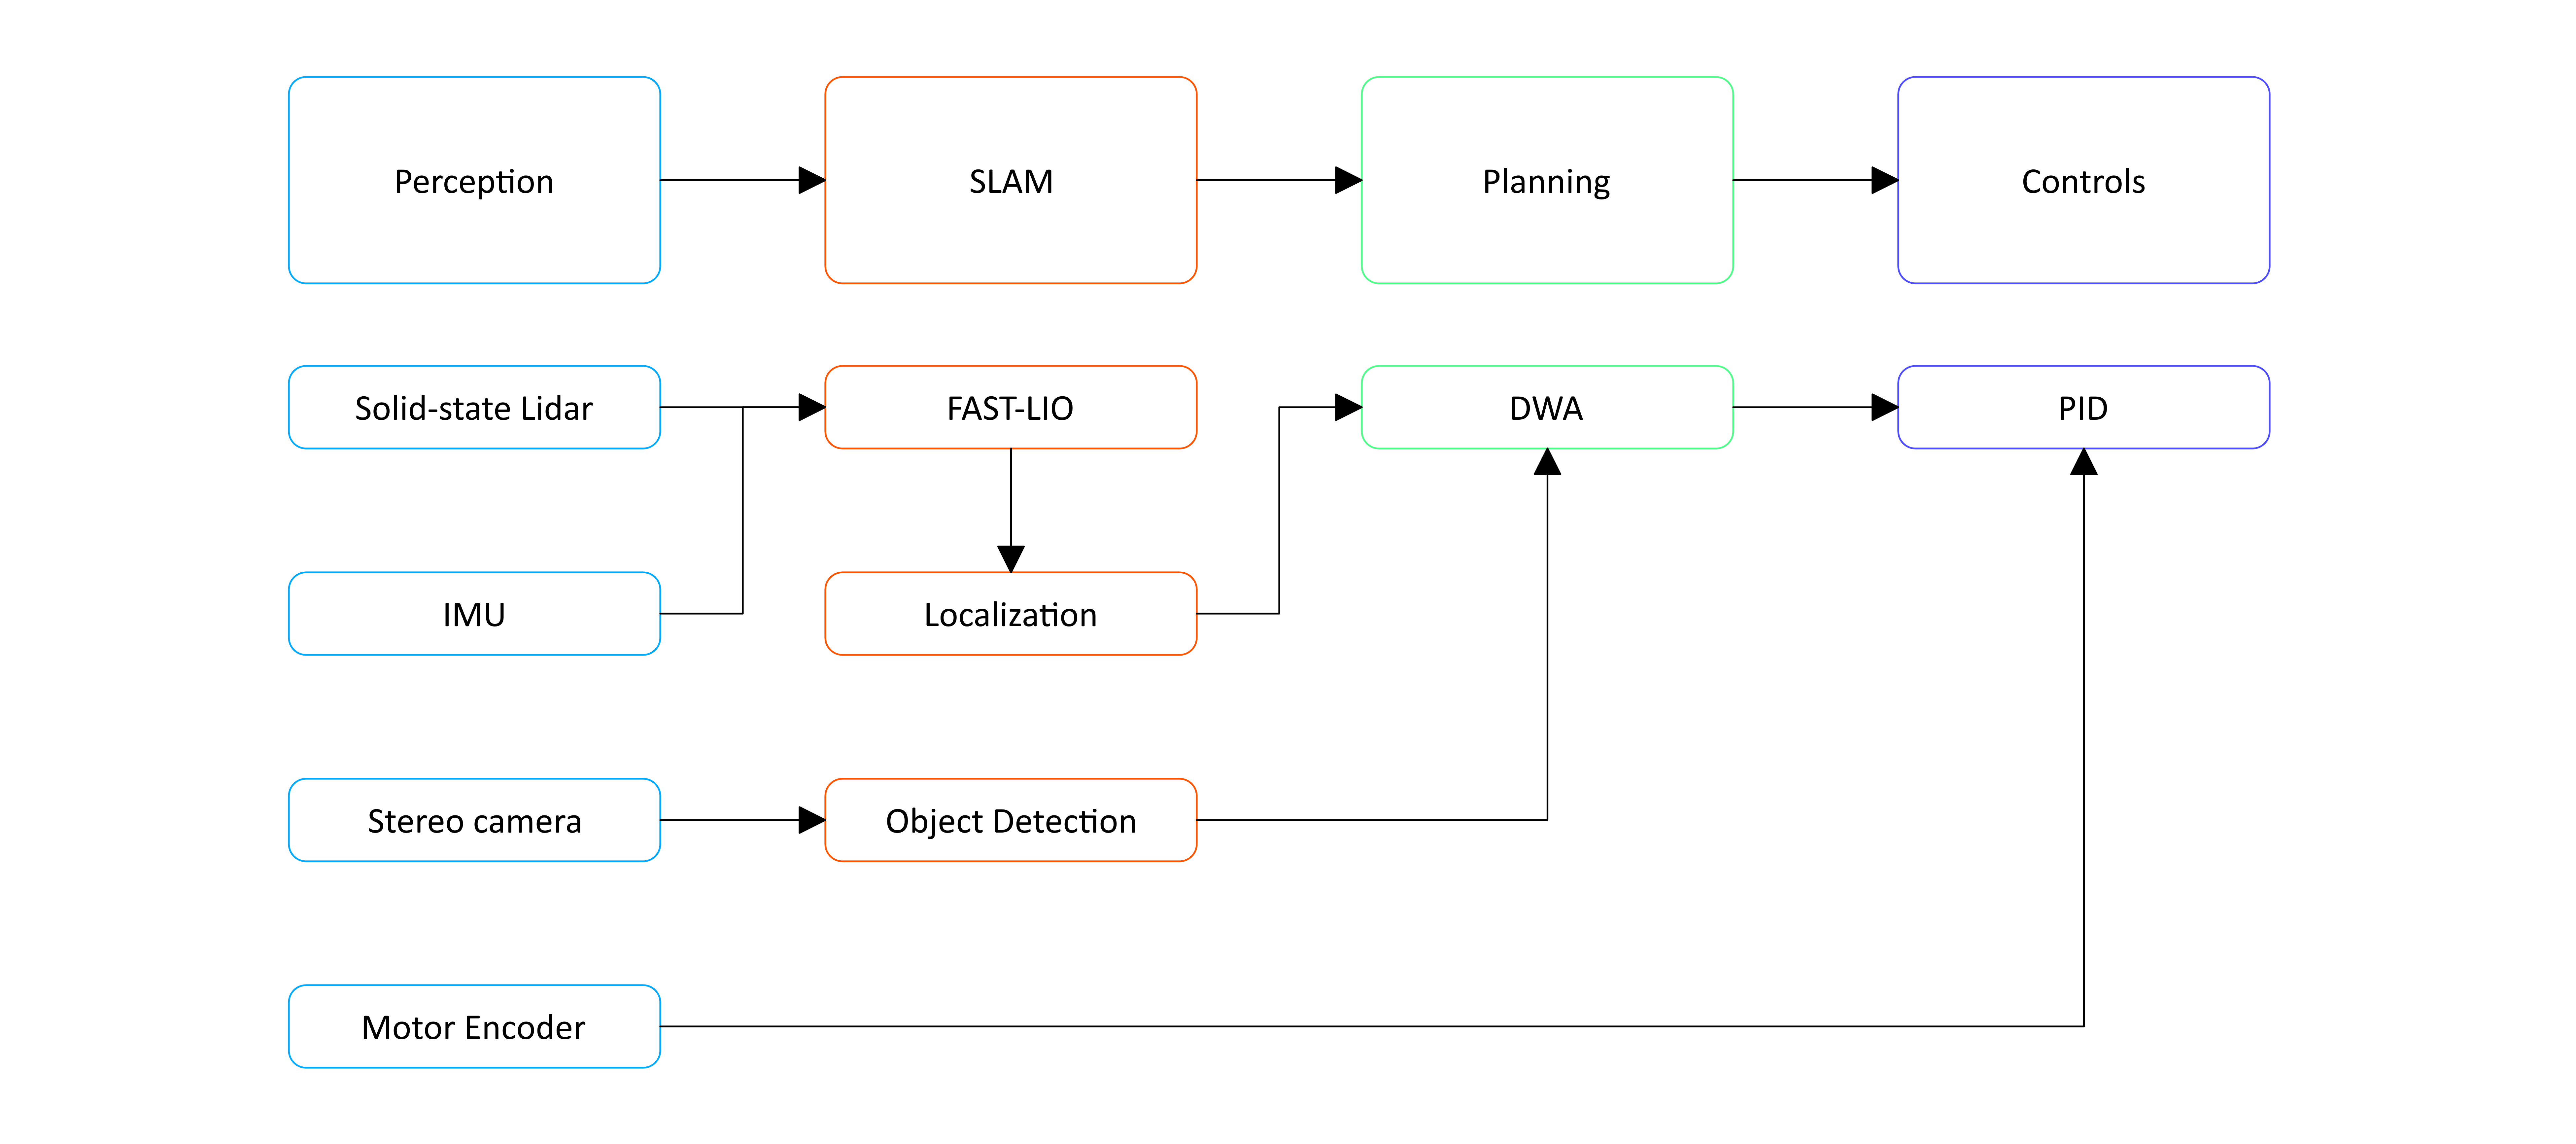
\includegraphics[width=0.9\textwidth]{flow_chart.png}
	\caption{flow chart}\label{flow}
	\end{figure*}
The over all work flow is shown in figure \ref{flow}. Before the actual experiment begins, the stereo camera is calibrated using the intrinsic matrix $K$ and the distortion coefficients $DC$, which are defined as:
\begin{equation}
	K=\left[\begin{array}{ccc}f_{x} & 0 & c_{x} \\ 0 & f_{y} & c_{y} \\ 0 & 0 & 1\end{array}\right]
\end{equation}
Where $f_x$ and $f_y$ are the focal length along $x$ and $y$ axis. $c_x$ and $c_y$ are the offsets of the principal axis.
\begin{equation}
	DC =\left[\begin{array}{lllll}k_{1} & k_{2} & p_{1} & p_{2} & k_{3}\end{array}\right]
\end{equation}
Such that the radio and tangential distortion are given as:
\begin{equation}
	\begin{aligned}
		&x_r=x\left(1+k_{1} r^{2}+k_{2} r^{4}+k_{3} r^{6}\right) \\
		&y_r=y\left(1+k_{1} r^{2}+k_{2} r^{4}+k_{3} r^{6}\right) \\
		&x_t=x+\left[2 p_{1} x y+p_{2}\left(r^{2}+2 x^{2}\right)\right] \\
		&y_t=y+\left[p_{1}\left(r^{2}+2 y^{2}\right)+2 p_{2} x y\right]
		\end{aligned}
\end{equation}
The corresponding parameters' values are shown in table \ref{calib}.

\begin{table}[!ht]
    \centering
    \begin{tabular}{p{0.3\linewidth} p{0.3\linewidth} p{0.3\linewidth}}
    \hline

	~ & Left lence & Right lence \\ \hline
	$f_x$ & 525.575 & 528.400 \\ 
	$f_y$ & 525.1050 & 527.8600 \\ 
	$c_x$ & 355.7350 & 627.9750 \\ 
	$c_y$ & 350.3825 & 370.8590 \\ 
	$k_1$ & -0.0408 & -0.0453 \\ 
	$k_2$ & 0.0081 & 0.0140 \\ 
	$p_1$ & 0.0000 & 0.0000 \\ 
	$p_2$ & 0.0000 & 0.0000 \\ 
	$k_3$ & -0.0041 & -0.0041 \\ \hline
    \end{tabular}
	\caption{Camera intrinsic parameters}\label{calib}
\end{table}

\paragraph{Perception} Besides the Solid-state lidar and the stereo camera, which is introduced in the previous section, there are 2 more sensors: the IMU and the motor encoder. The IMU is used to measure the dynamic properties of the robot. For example the acceleration and the angular acceleration. The veolcity and the estimated position can be obtained by integrating the acceleration. It should be noticed that the position obtained here can not be used directly because there is drifts due to the intrinsic noise of the IMU, hence the point cloud matching localization of the lidar is necessary. The motor encoder is used to measure the rotational speed of the wheels so that the commanded speed can be maintained using a PID control policy.
\paragraph{Simultaneously Localization and Mapping} There are 2 sensors in charge of the localization process: the IMU and the lidar. The IMU is stable as long as there is no strong magnetic field around. It will never be influenced by the surrounding obstacles. However, it will have large drift upon small errors of the accelerometer. On the other hand, the lidar point cloud matching method will correct it self when more points are detected. However, the lidar is very sensitive with respect to the envirnonment. Given the pros and cons of these 2 sensors. The final localization is done by merging these 2 sensors' data using the Kalmen filter.
Figure \ref{path_plan2} shows the cost map of the route between CMU's Hunt library and gym.  
\paragraph{Planning} The planning is divided into global planning and local planning. The global planning is done by using the A* algorithm and the local planning is done by DWA algorithm. The A* algorithm is a breath first search based method with weights added to each steps of the exploration. The Dynamic Window Approach is a local planning method that searches the robot control space $u$, where:
\begin{equation}
	u=\left[\begin{array}{c}\dot{x}\\\dot{y}\\\dot{\theta}\end{array}\right]
\end{equation}
\paragraph{Control} The control is done by using the PID control policy. The PID control policy is a feedback control policy that is used to maintain the speed of the robot.
%%%%%%%%%%%%% begin figure %%%%%%%%%%%%%%%%%

%% captions go below figures

\begin{figure}
\centering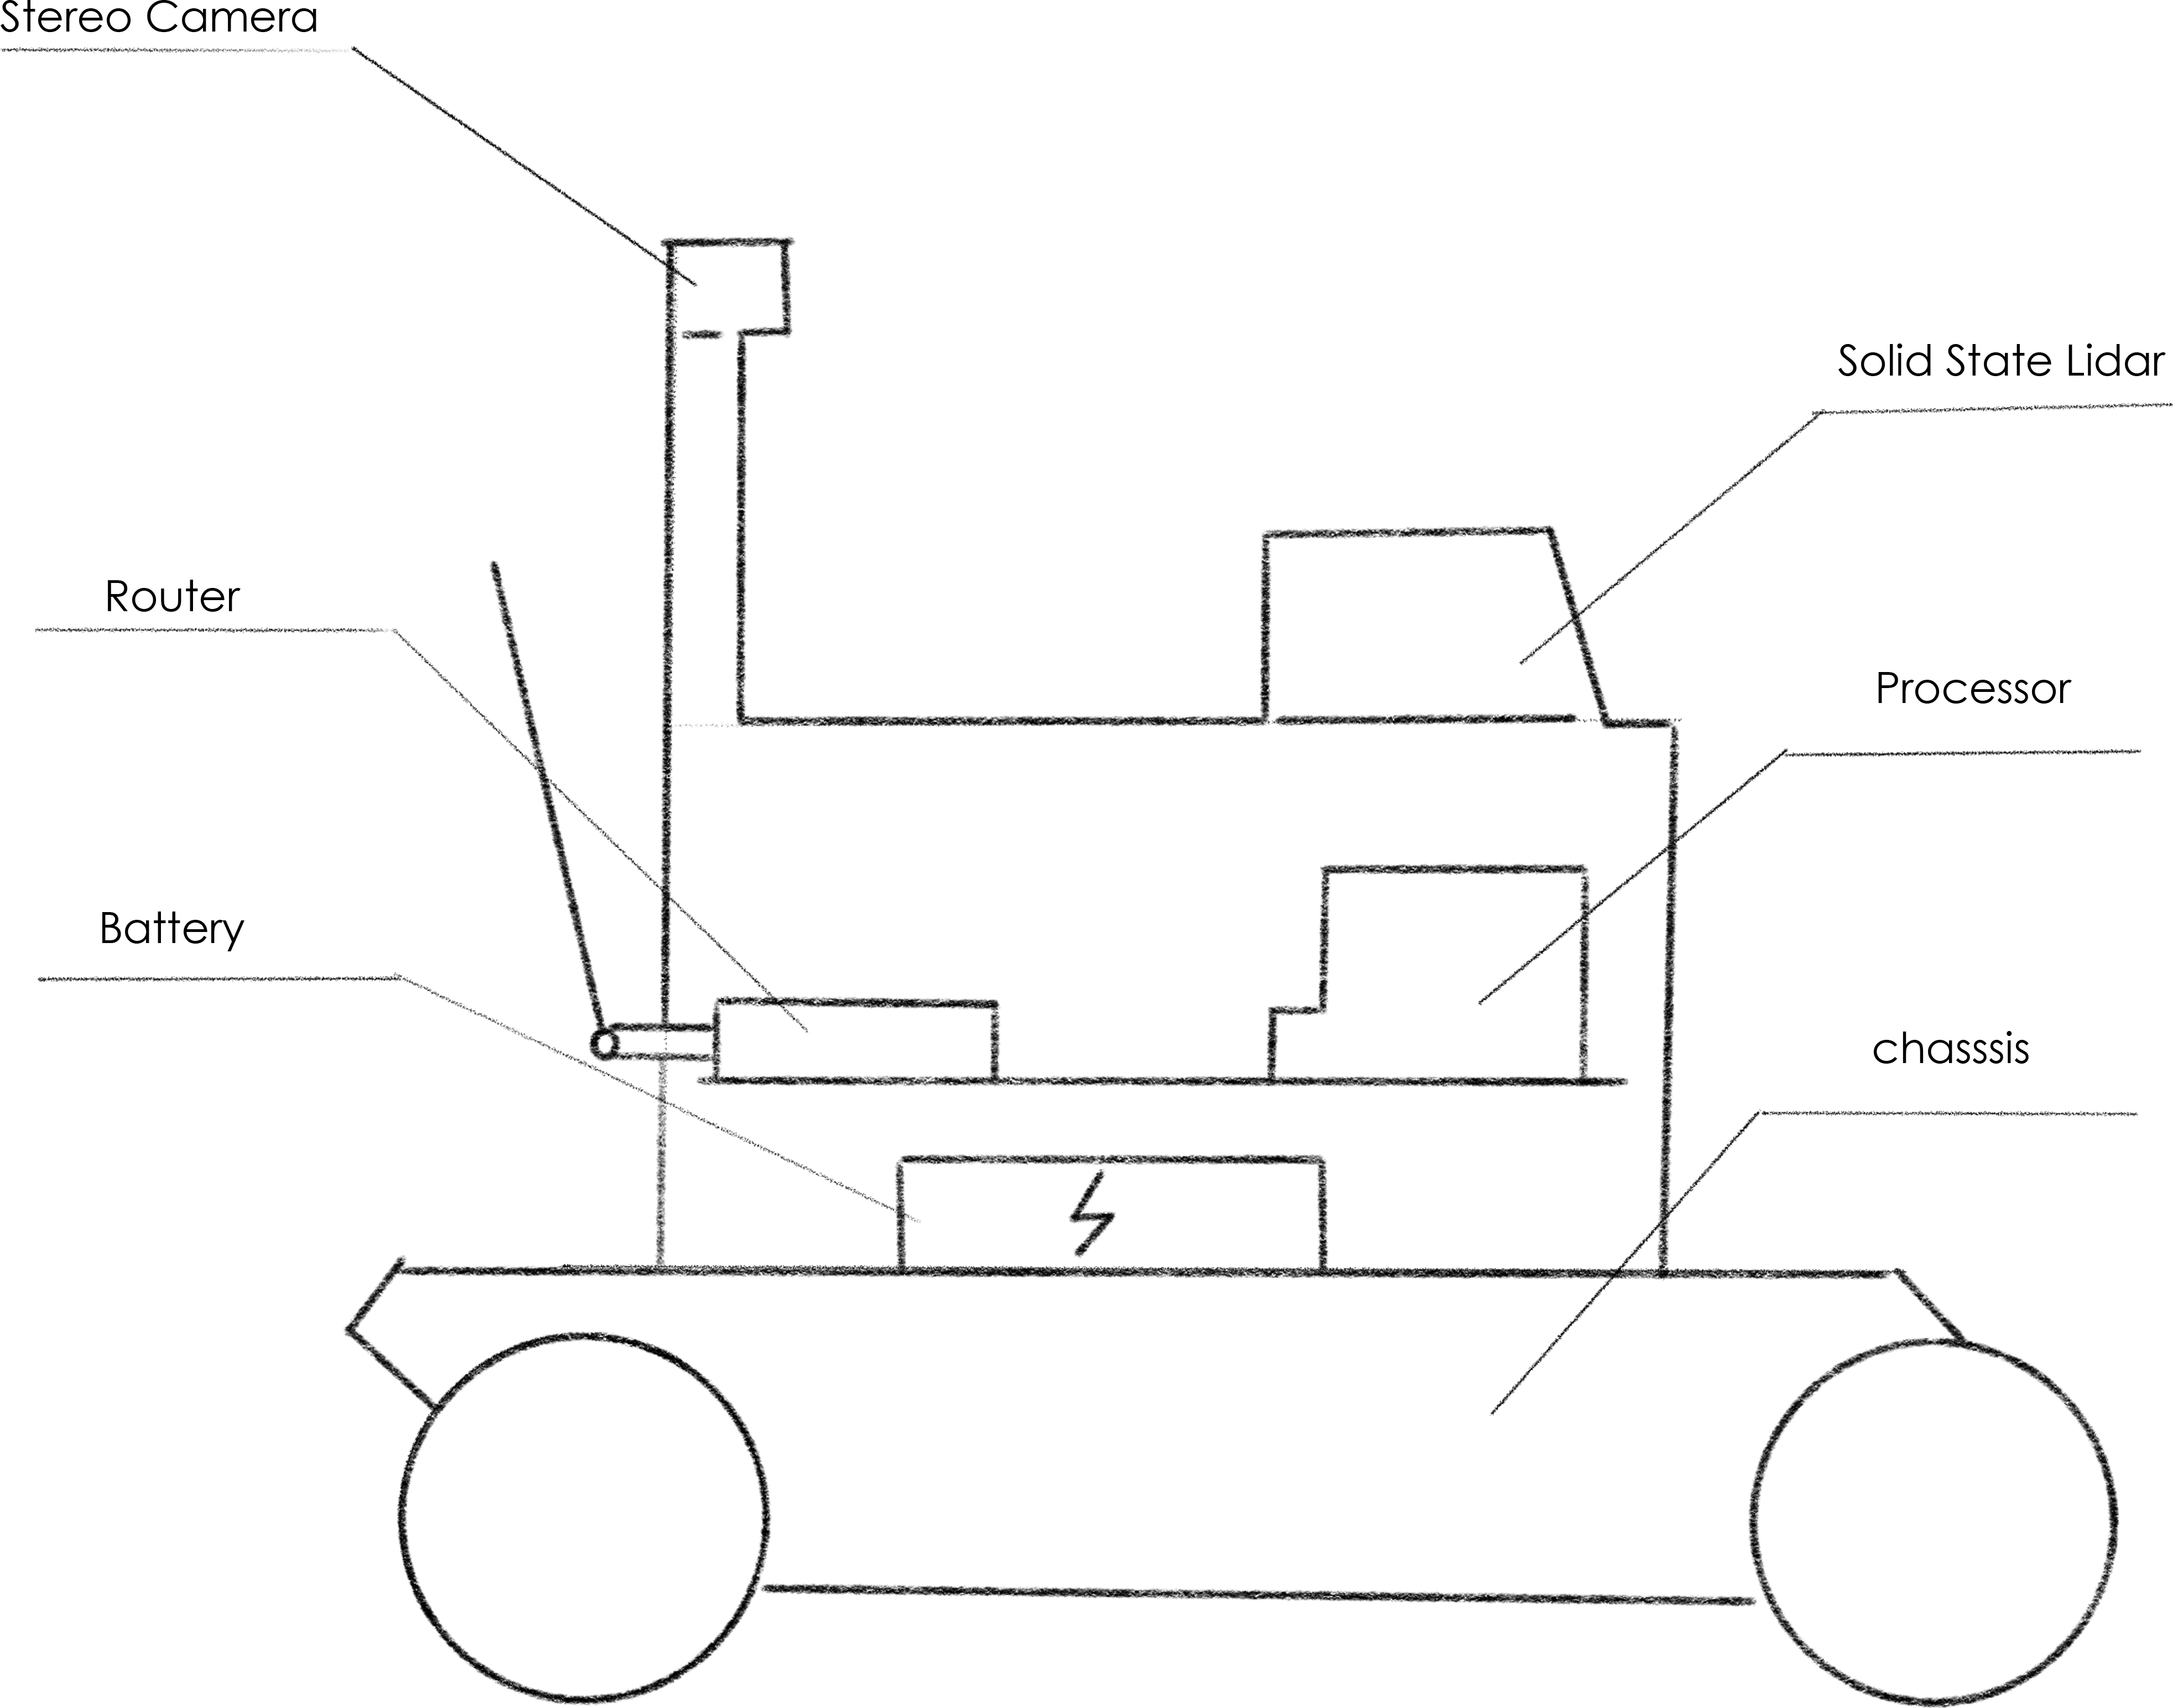
\includegraphics[width=0.7\linewidth]{system.png}
\caption{System design}\label{sys}
\end{figure}

\begin{figure}
\centering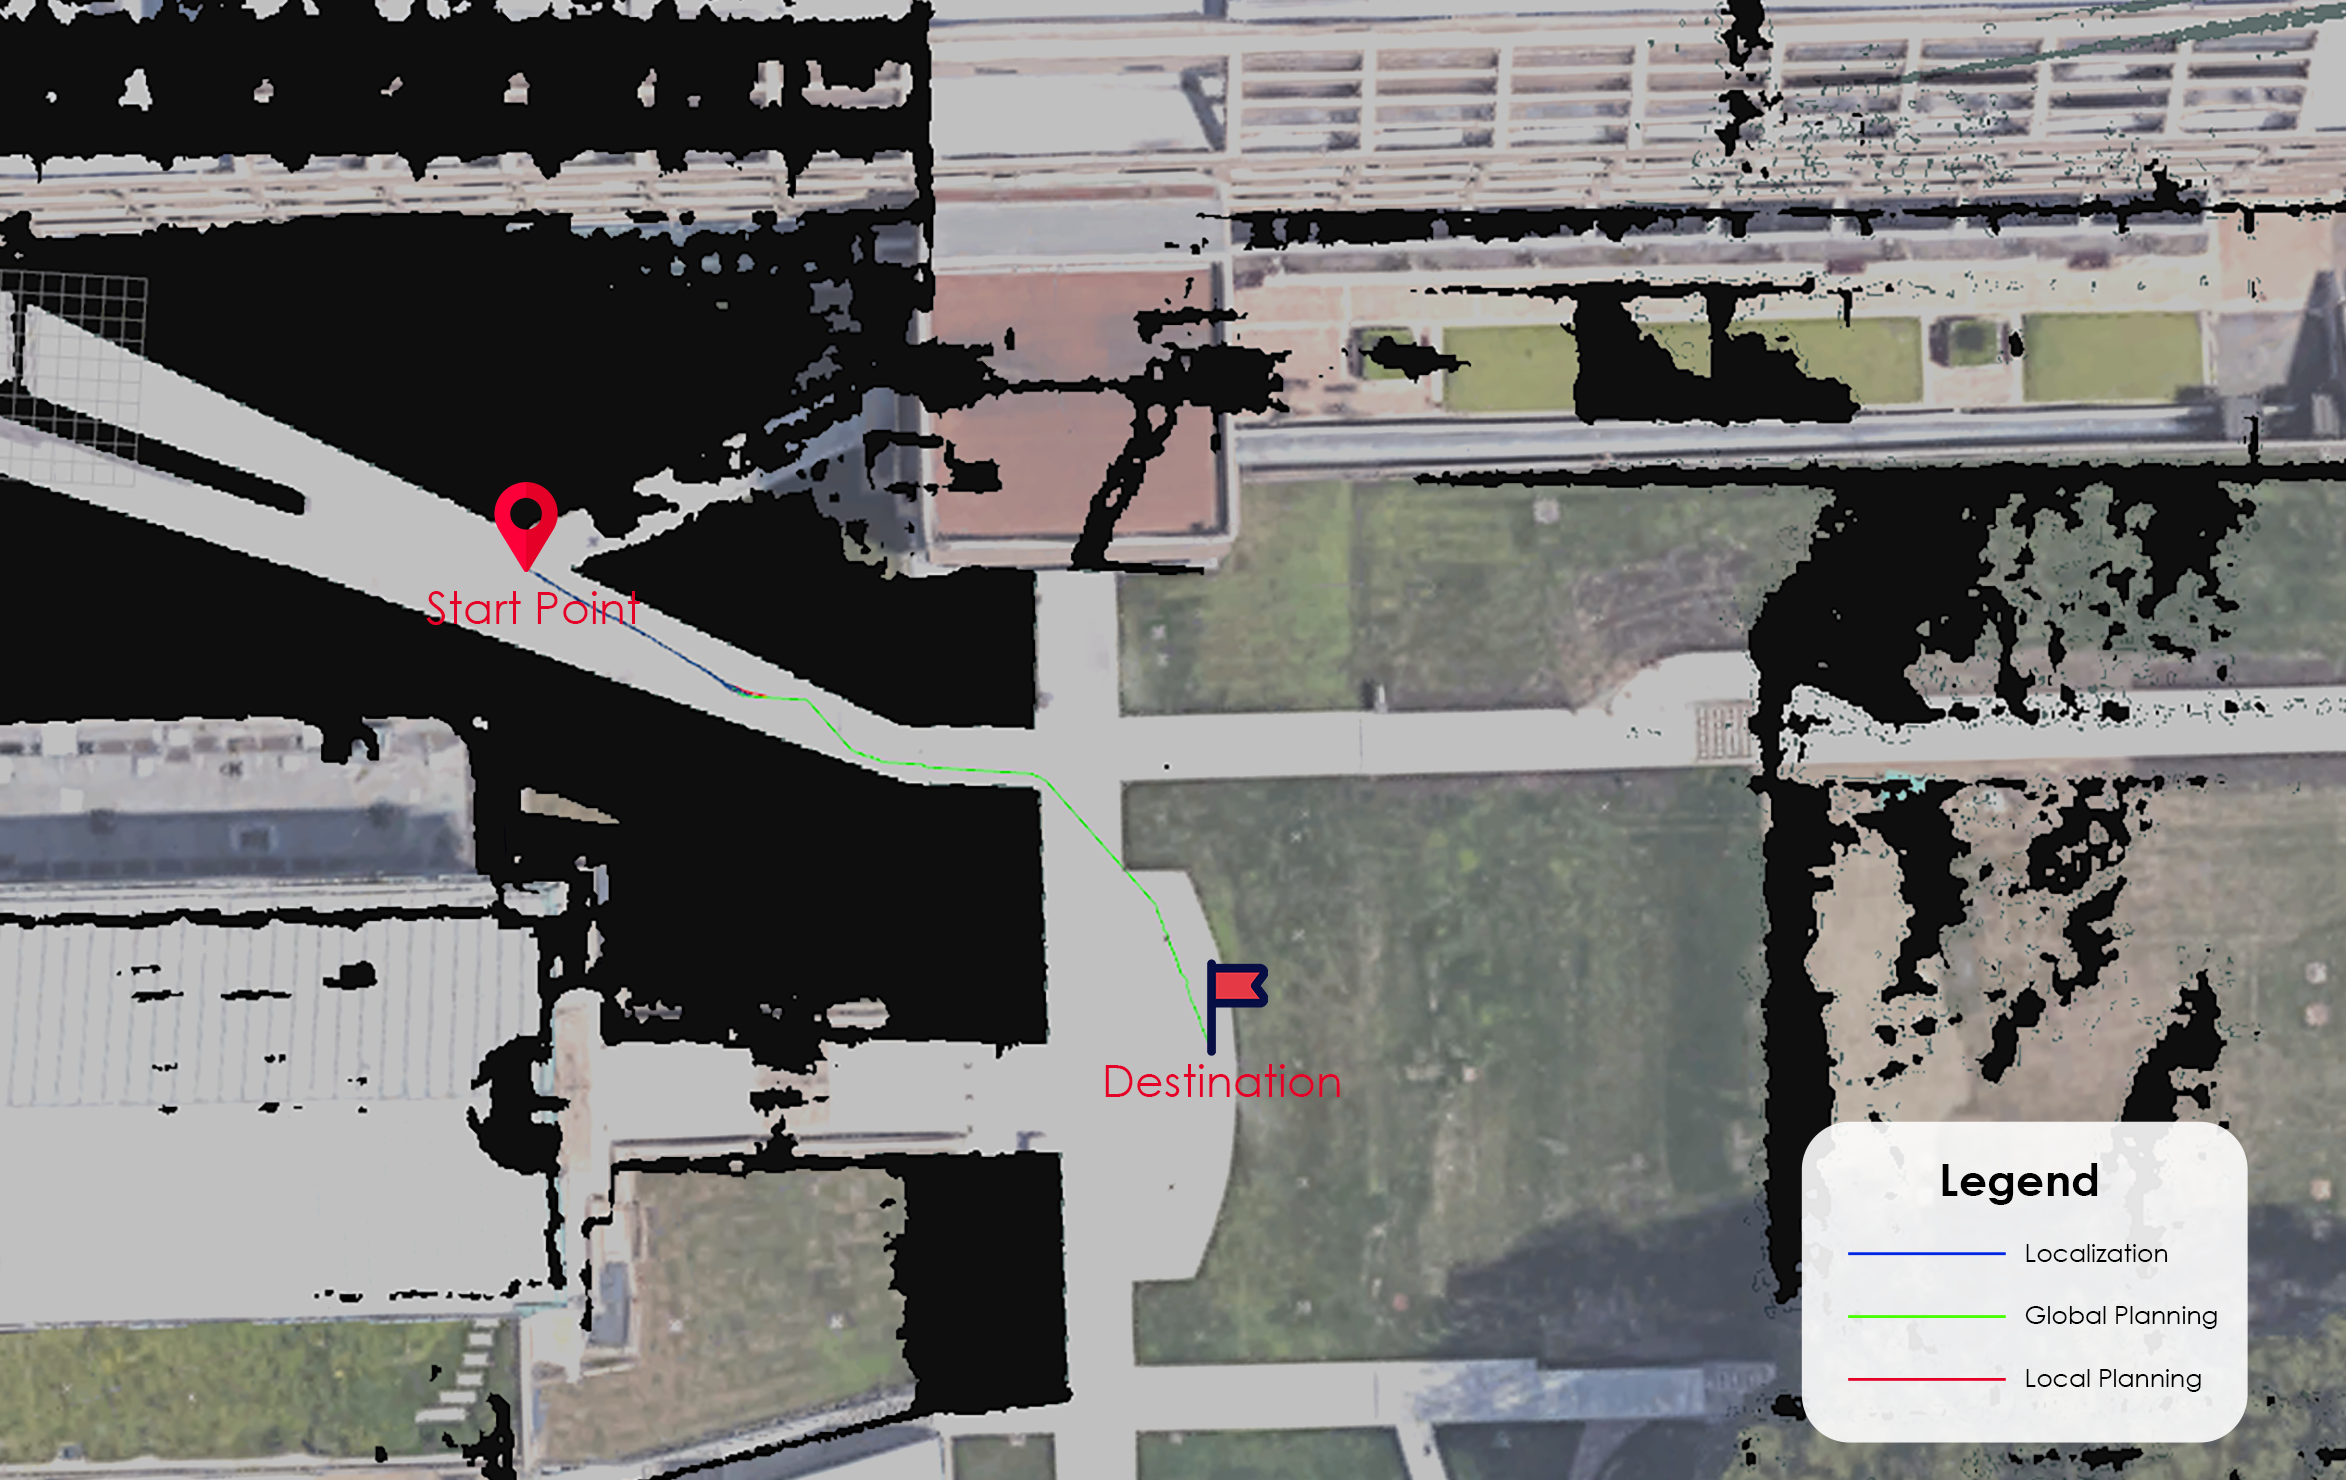
\includegraphics[width=0.7\linewidth]{Planning_psed.png}
\caption{Cost map}\label{path_plan}
\end{figure}

\begin{figure}
	\centering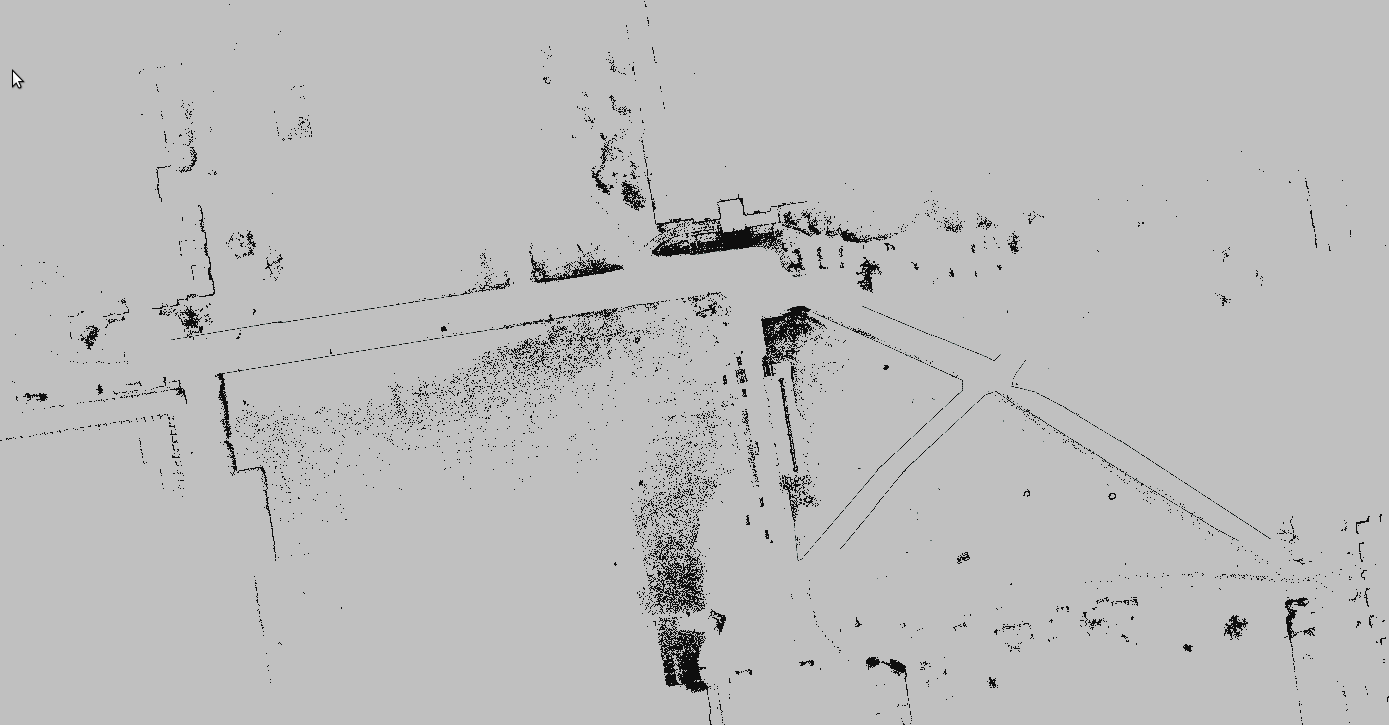
\includegraphics[width=0.7\linewidth]{Hunts_UC_2D.png}
	\caption{Cost map for another route}\label{path_plan2}
	\end{figure}
 
\begin{figure}
\centering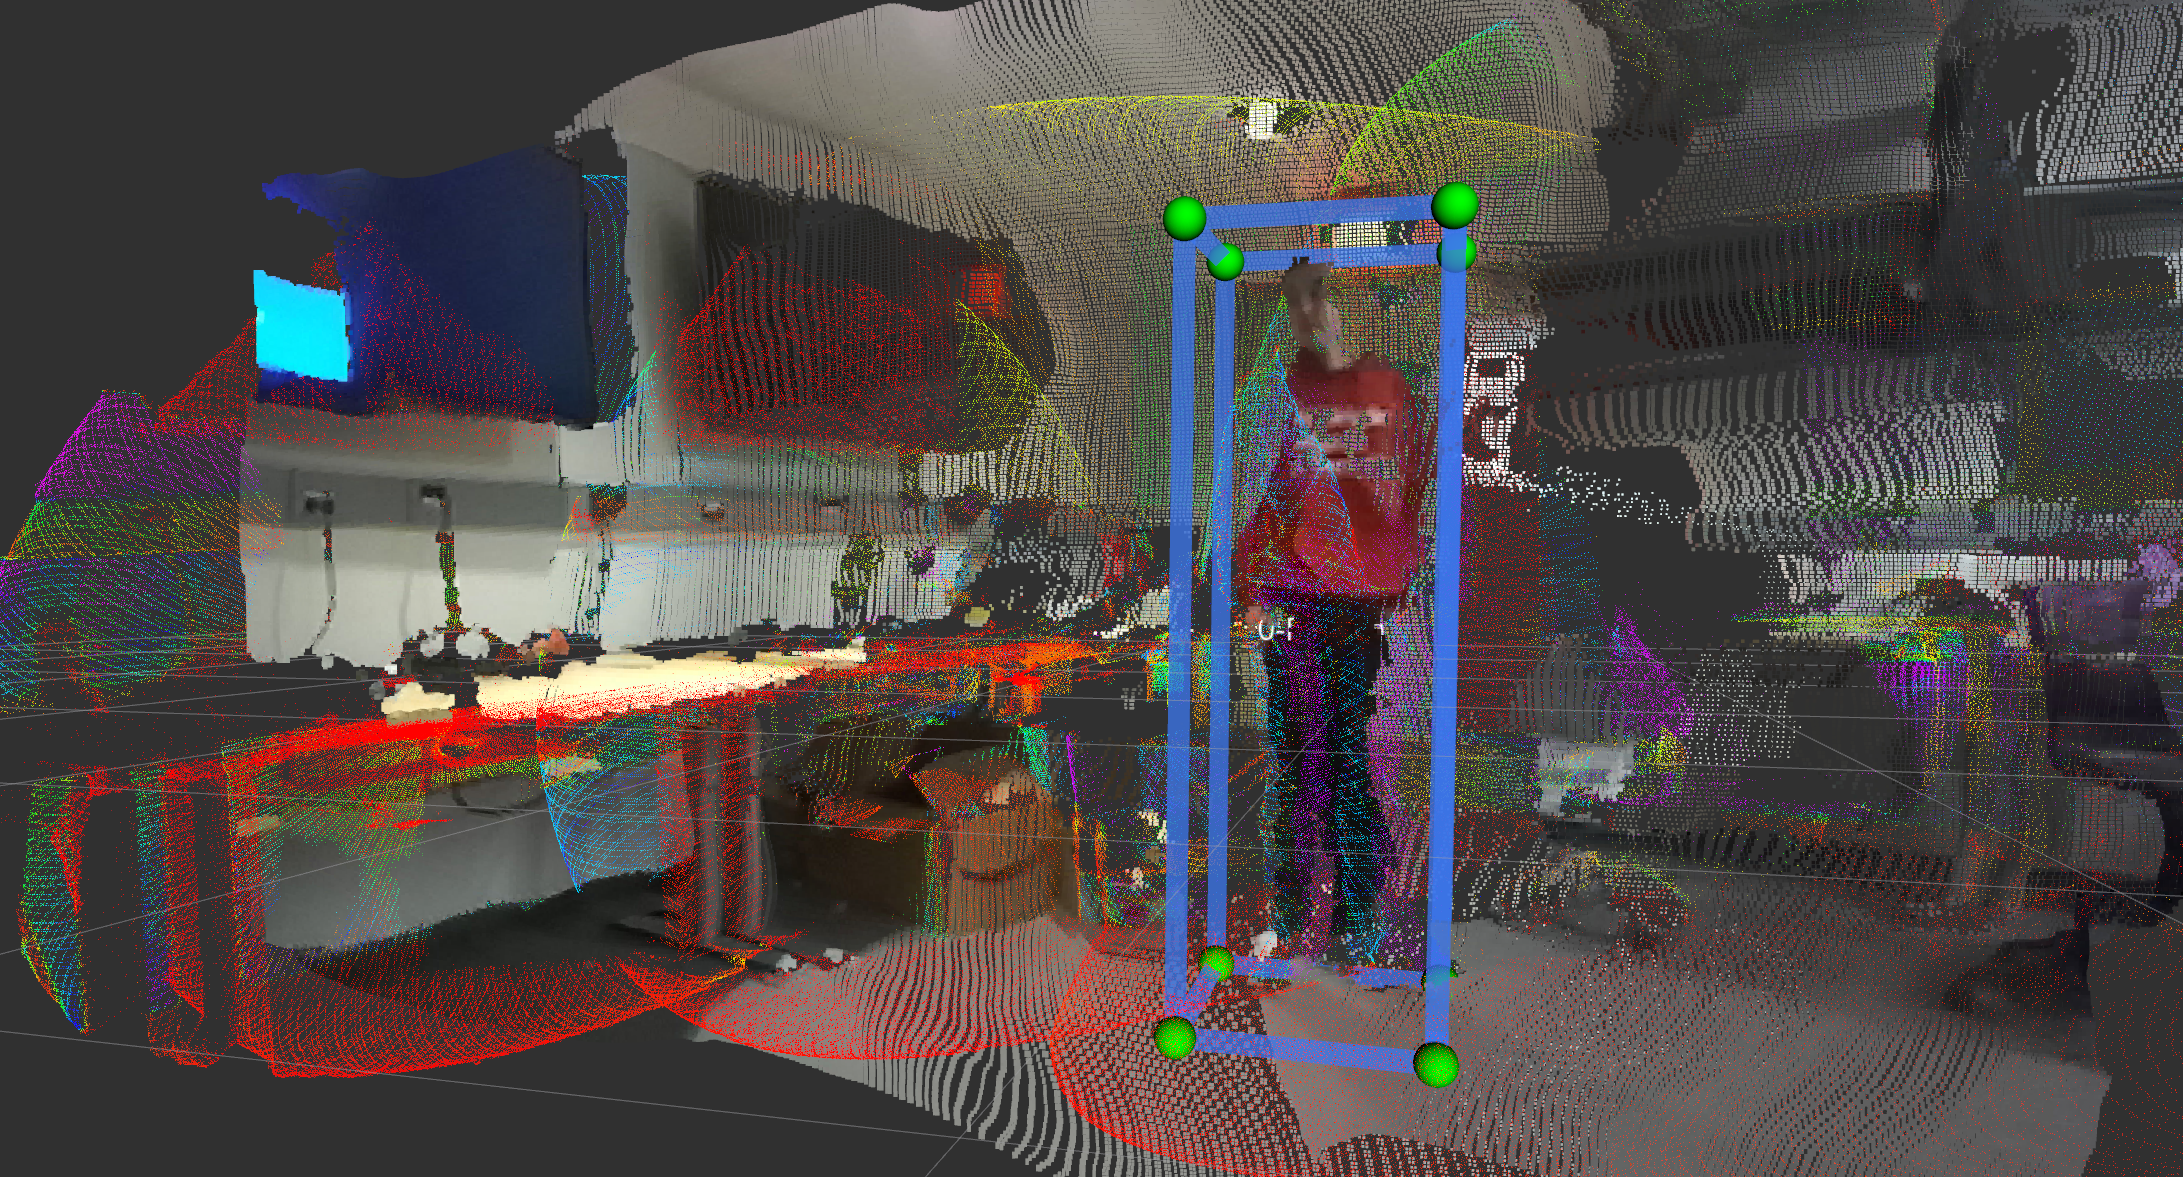
\includegraphics[width=0.7\linewidth]{obj_det.png}
\caption{Object detection verified by lidar}\label{obj_det}
\end{figure}




\begin{figure*}
	\center
	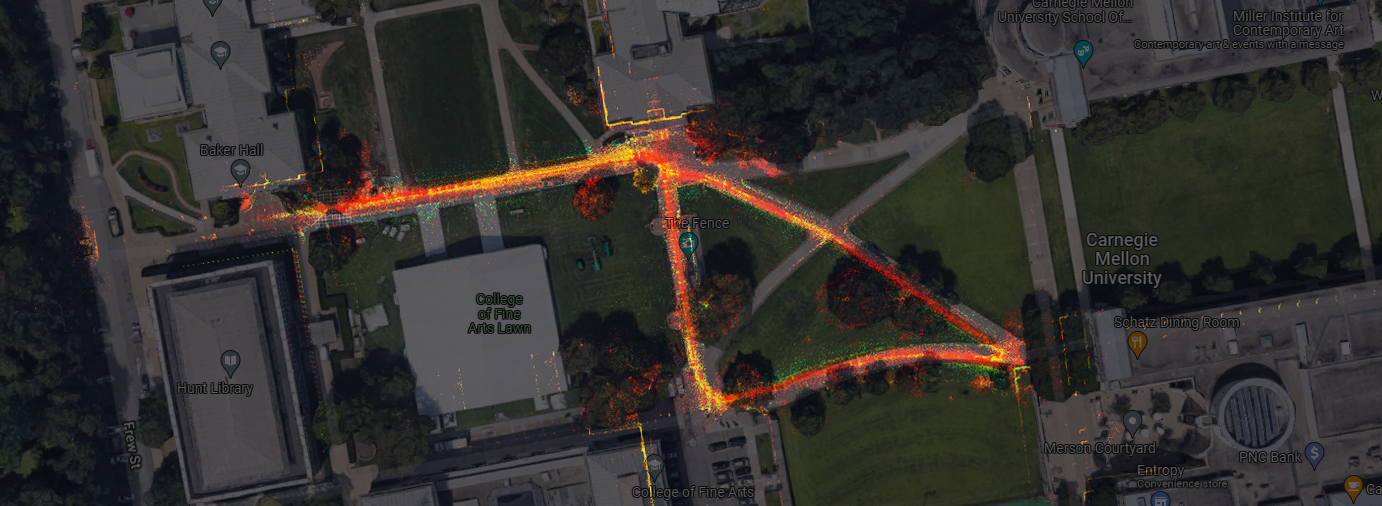
\includegraphics[width=0.9\textwidth]{map_psed_hunt.png}
	\caption{Comparison with google map}\label{hunt}
	\end{figure*}


%%%%%%%%%%%%% end figure %%%%%%%%%%%%%%%%%%%


%%%%%%%%%%%%%%%%%%%%%%%%%%%%%%%%%%%%%%%%%%%%%%%%%%%%%%%%%%%

%% Use title case for subsections and subsubsections (first letter of words capitalized)

\section{Results}

Figure \ref{obj_det} shows 2 views of the stereo camera object detection result of a person. The results are shown in blue bounding box with green vertices. The strips in the figures are the lidar point cloud. It is shown that the person in the bounding box is closely surrounded by the strips, which shows that the lidar point cloud overlaps with the camera object detection. Figure \ref{path_plan} shows the planning result of the vehicle. The green line is the global planning path, the red line is the local planning path and the blue line is the localization.

According to the figures, the stereo camera’s object detection is relatively accurate even under indoor
envirnonment. The lidar’s point cloud is also shown to have a very good alignment with the depth map given by
the stereo camera.
%%%%%%%%%%%%%%%%%%%%%%%%%%%%%%%%%%%%%%%


%%%%% Acknowledgments %%%%%%%%%%%%%%%%%%%%%%%%%%%

\section*{Acknowledgments}

Thanks to Professor Ding and all members in the team of Safe AI Scout at Safe AI Lab, the system of our prototype is developed in a very smooth way. I am very grateful to the members of the team not only for their hard work and dedication but also for their suggestions and feedbacks. 

The time at Safe AI Lab is very valuable. Not only did I established the software and hard ware system for an autonomous delivery robot, but also I got the opportunity to learn the techniques in order for a real world system to work. For example the software environment and the hardware environment are very important for the software development. Sometimes we spent days on the compatibility between software packages. I also learned that the cooling system is very important for the performance of the robot.

I also want to say thank you to my mentors for their high level guidance for what the whole architecture of an autonomous robot will be like. This gives us a very clear idea of how to build a robot at the very beginning of our development. 

%%%  REFERENCES  %%%%%%%%%%%%%%%%%%%%%%%%%%%%%%%%
%%
%% Put your references into your .bib file in the usual way. Run latex once, bibtex once, then latex twice.
%% The asmeconf.bst style allows @inproceedings and @proceedings to include: 
%%		venue = {Location of Conference}, 
%%		eventdate = {Month, days},

\nocite{*}%% <=== Delete this line unless you want to typeset the entire contents of your .bib file!

\bibliographystyle{asmeconf}  %% .bst file following ASME conference format. Do not change.
\bibliography{asmeconf-sample}%% <=== change this to name of your bib file


%%%  APPENDICES  %%%%%%%%%%%%%%%%%%%%%%%%%%%%%%%%
\appendix

%% Note that appendices will be "numbered" A, B, C, ... etc. Use \section, not \section*
%% Equations will be numbered sequentially following those in the paper. Do not reset the equation counter.

%% Here we use the optional argument to control the pdf bookmark and prevent errors.
\newpage
\section[Camera Lidar Calibration]{Codes for Camera Lidar Calibration}\label{appendix:a}

\begin{minted}[linenos,tabsize=2,breaklines]{python} 
import pyzed.sl as sl # Import the stereo camera's library
import cv2 # Import OpenCV
init_params = sl.InitParameters() # Create a sl.InitParameters object
init_params.camera_resolution = sl.RESOLUTION.HD2K # Use HD2K resolution
zed = sl.Camera() # Create a camera object
zed.open(init_params) # Open the camera
if not zed.is_opened(): # Check if camera opened successfully
	exit()
print("Opening ZED Camera...") # Remind the user that the camera is opening
zed.grab(init_params) # Grab a new image
image = sl.Mat() # Create a sl.Mat object

zed.retrieve_image(image) # Retrieve the left image
cv2.imwrite("test.png", image.get_data()) # Save the image
\end{minted} 

%%%%%%%%%%%%%%%%%%%%%%%%%%%%%%%%%%%%%%%%%%%%%%%%%%%%%%%%%%%%%%%%%%%%%%%%%%%%%%%%%%%%%%%

\end{document}

